\documentclass[master=arc,british,oneside]{kulemt}
\ExpandArgs{NNo}\newcommand*\classversion{\fileversion}
\newcommand*\manualdate{2025-02-22}
\setup{title={Writing a Master's Thesis in LaTeX},
  subtitle={The `kulemt' v\classversion\ manual (\manualdate)},
  author={Luc Van Eycken},
  promotor={Prof.\,dr.\,ir. M.~Schevenels},
  assessor={Werkgroep masterproef},
  assistant={P. Wilson \and D. Knuth}}

%% Fonts 
%  - Select the main text and math fonts
%    Remember their names, so we can use them in the text
\usepackage{libertinus}
\newcommand*\rmfontname{Libertinus Serif}
\newcommand*\sffontname{Libertinus Sans}
\IfPackageLoadedTF{fontspec}%
  {%
    \usepackage{unicode-math}%
    \setmathfont{Libertinus Math}%
    \setmonofont{Latin Modern Mono}%
    \newcommand*\ttfontname{Latin Modern Mono}%
  }%
  {%
    \usepackage{libertinust1math}%
    \renewcommand{\ttdefault}{lmtt}%
    \newcommand*\ttfontname{Latin Modern Typewriter}%
    \DeclareUnicodeCharacter{1EBF}{\'{ê}}% For "Hàn Thế Thành"
  }
%  - Use microtype to enhance the typography
\usepackage{microtype}
%  - Generate an error for missing glyphs
\tracinglostchars=3

%% Biblatex for citations and annotated bibliography
\usepackage[style=numeric,abbreviate=false]{biblatex}
\addbibresource{refs.bib}
\DeclareFieldFormat{url}{\newline\nobreak\mkbibacro{URL}\addcolon\space\url{#1}}
\renewbibmacro*{urldate}{} % Do not print urldate
\DeclareFieldFormat{texdoc}{%
  Local documentation: \textcolor{teal}{\ttfamily texdoc #1}}
\DeclareFieldFormat{annotation}{#1}
\renewbibmacro{finentry}{\setunit{\finentrypunct}%
  \setunit{\par\nobreak}%
  \printfield{texdoc}%
  \setunit{\par\nobreak}%
  \printfield{annotation}%
  \finentry}
\DeclareSortingTemplate{nty}{%
  \sort{\field{presort}}%
  \sort[final]{\field{sortkey}}%
  \sort{% Entries with a missing name come first
    \field{sortname}%
    \field{author}%
    \field{editor}%
    \field{translator}%
    \literal{0}}%
  \sort{%
    \field{sorttitle}%
    \field{title}}%
  \sort{%
    \field{sortyear}%
    \field{year}}%
  \sort{%
    \field{volume}%
    \literal{0}}}
\newcommand*\citewithtitle[2][]{\citetitle{#2}~\cite[#1]{#2}}
\usepackage{metalogox}  % Better formatting of TeX, ... in bibliography

%% Additional formatting settings
%  - Use the chapter and headings styles as well as the ToC formatting
%    and the KU Leuven conventions as defined in the kulemtx document style.
%    Additionally it defines some extra user commands.
\usepackage[manual]{kulemtx}
%  - Lists are tighter than default
\firmlists
%  - Footnotes: set the marker flushleft and the text as a block paragraph
\setlength\footmarkwidth{1.5ex}
\setlength\footmarksep{0pt}
\footmarkstyle{\textsuperscript{#1}\hfill}
%  - URLs: Using \textlangle instead of \langle because \langle gives problems
%    under luatex with certain fonts (e.g. Latin Modern Mono).
\usepackage{url}
\ExplSyntaxOn
\cs_set_nopar:Npn \UrlLeft #1 \UrlRight{
  \tl_set:Nn \l_tmpa_tl {#1}
  \regex_replace_once:nnN { \A https?:// } {} \l_tmpa_tl
  \regex_replace_once:nnN { / \Z } {} \l_tmpa_tl
  \hbox:n { \rmfamily \small \textlangle }
  \l_tmpa_tl
  \hbox:n { \rmfamily \small \textrangle }
}
\ExplSyntaxOff

%% Additional packages
%  - subfigures
\newsubfloat{figure}
%  - tikz/pgf
%    Note: also loads xcolor
\usepackage{tikz}
\usetikzlibrary{arrows,calc}
%  - csquotes (needed by biblatex) !!! TODO: use it
\usepackage{csquotes}

%% Finally hyperref is loaded for proper PDF links
%  Colors: external links in blue, internal ones in dark blue
\usepackage[pdfusetitle,bookmarksnumbered]{hyperref}
\hypersetup{colorlinks,%
  filecolor={[rgb]{0,0,1}},urlcolor={[rgb]{0,0,1}},%
  citecolor={[rgb]{0,0,.75}},linkcolor={[rgb]{0,0,.75}}}
\pdfstringdefDisableCommands{\let\cs\textbackslash}

%% Define some typesetting commands
%  NOTE: Please don't use logos (\LaTeX ...) in the text, but simply LaTeX ...
\newcommand*\acro[1]{{%
    \ifdim\csname f@size\endcsname pt<10pt\else \expandafter\small\fi #1}\@}
\newcommand*\cls[1]{\textsf{#1}}
\newcommand*\pkg[1]{\textsf{#1}}
\newcommand*\env[1]{\cmdprint{#1}}
\newcommand*\opt[1]{\texttt{#1}}
\newcommand*\file[1]{\texttt{#1}}
\newcommand*\prog[1]{\texttt{#1}}
\newcommand*\PDF{\acro{PDF}}
\newcommand\Dutch[1]{`\foreignlanguage{dutch}{#1}'}
\newcommand\English[1]{`\foreignlanguage{english}{#1}'}
\newcommand*\NewInVersion[1]{%
  \sidepar{\small\textcolor{gray}{New in v#1}}\ignorespaces}

\begin{document}

\begin{preface}
  I would like to thank everybody who has kept me busy with writing, debugging,
  and documenting this LaTeX document class. My thanks goes especially to my
  supervisor and my assistant-supervisors. I also thank my assessors, at least
  those who read this text.

  Finally I would like to thank all the people who provided feedback,
  either with bug reports or by suggesting improvements.
\end{preface}

\tableofcontents

\begin{abstract}
  This document describes the use of the LaTeX document class \cls{kulemt},
  which implements the KU~Leuven Faculty of Engineering Science guidelines for
  writing a master's thesis. Since there are slight differences between the
  actual guidelines of the different engineering master's programmes, this
  class implements not only the common part, but it also provides the necessary
  options to adapt it to the specific requirements. So please check the
  guidelines of your master's programme before using or tweaking typesetting
  options.

  To illustrate the difference between the main text language and the master's
  programme language, this document is written in English (as the main text
  language) for a Dutch master's programme.

  This manual (dated \manualdate) describes the \cls{kulemt} class
  version~\classversion.
\end{abstract}

\begin{abstract*}
  Dit document beschrijft de LaTeX-documentklas \cls{kulemt}, die de
  richtlijnen van de Faculteit Ingenieurswetenschappen van de KU~Leuven
  voor het schrijven van een masterproeftekst implementeert. Maar vermits
  de richtlijnen van de verschillende ingenieursopleidingen licht
  verschillen, voorziet de documentklas de nodige opties om het resultaat
  aan te passen. Hou dus bij het aanmaken van de tekst niet zozeer rekening
  met wat de documentklas toelaat, maar wel met wat jouw master als
  specifieke richtlijnen opgeeft.

  Voor studenten van een Nederlandstalige master die hun masterproef in het
  Engels schrijven (bv.\ Erasmus-studenten) is een Nederlandse samenvatting
  verplicht. Als jouw master een uitgebreide samenvatting verlangt met
  figuren en tabellen kun je die best voorzien als een bijlage. Anders
  volstaat deze samenvatting van 1~bladzijde.

  Om het effect van twee talen te illustreren is dit document geschreven
  als een Engelse tekst (verder \English{text language} genoemd) voor een
  Nederlandstalige master (verder \English{master's programme language}
  genoemd).

  Deze handleiding van \manualdate\ beschrijft de LaTeX-documentklas
  \cls{kulemt} versie~\classversion.
\end{abstract*}

\listoffiguresandtables

\mainmatter

\chapter{Writing a thesis in LaTeX}
A LaTeX document class has been developed, which follows the guidelines
described in \cite{kulemtgl}. The usage of this class is described in
\Cref{cha:kulemt}. \Aref{app:template} contains a typical LaTeX template. The
result can be customised and adapted to the master's programme guidelines with
the class options. Additional functionality is available through numerous LaTeX
packages (cf.\ \Sref{sec:packages}). Just make sure that the final result still
conforms to the guidelines.

The following sections assume you already have a working LaTeX installation. If
this is not the case on a Linux based distribution, first check the
distribution documentation. Otherwise consult the TeX-FAQ\,\cite{texfaq} for
installing a LaTeX distribution for your system.

If you are not (yet) familiar with LaTeX, you should first have a look at the
documentation of the TeX Users Group \cite{tugstart}. It also contains a list
of on-line tutorials and manuals. The most popular tutorial is probably
\citewithtitle{lshort}. The next section contains some extra information on how
to install LaTeX packages. It also lists some typically useful packages.

\section{Using LaTeX packages}\label{sec:packages}
The document class \cls{kulemt} uses some standard LaTeX packages (such as
\pkg{babel} and \pkg{graphicx}) and is based on the document class
\cls{memoir}, so it also includes all packages included or emulated by
\cls{memoir}\,\footnote{The \cls{memoir} class includes or emulates since
  2018-12-12 at least the packages \pkg{abstract}, \pkg{appendix}, \pkg{array},
  \pkg{booktabs}, \pkg{ccaption}, \pkg{changepage}, \pkg{chngcntr},
  \pkg{chngpage}, \pkg{crop}, \pkg{dcolumn}, \pkg{delarray}, \pkg{enumerate},
  \pkg{epigraph}, \pkg{ifmtarg}, \pkg{index}, \pkg{makeidx}, \pkg{moreverb},
  \pkg{mparhack}, \pkg{needspace}, \pkg{newfile}, \pkg{nextpage},
  \pkg{pagenote}, \pkg{parskip}, \pkg{patchcmd}, \pkg{setspace},
  \pkg{shortvrb}, \pkg{showidx}, \pkg{tabularx}, \pkg{titleref}, \pkg{titling},
  \pkg{tocbibind}, \pkg{tocloft}, \pkg{tocvsec2}, \pkg{verbatim}, and
  \pkg{verse}.}. The exact list of packages included or emulated in
\cls{memoir} can always be found in the log file after a LaTeX run. The
emulation not always corresponds to the latest version of the package, but the
main functionality is usually present. So before installing a new package,
first check the \cls{memoir} manual\,\cite{memman} to see if the functionality
is not already present in the document class.

\subsection{Installing a LaTeX package}\label{sec:install}
Most of the packages listed below are included in a standard LaTeX
installation, with the exception of the \pkg{kulemt} package. But in case you
need to install a package yourself, you can follow the instructions found in
the TeX-FAQ\,\cite{texfaq} under the heading \enquote{Shortcuts to installing
  files}. If you only can or want to install packages for your personal use,
make sure you also read \enquote{Private installations of files}.

The installation of the document class \cls{kulemt} is done in the same way as
the installation of any other package. The only difference is the fact that its
source is currently not available from \acro{CTAN} or a Linux distribution but
from a local web server\,\citeurl{pkg:kulemt}.

\subsection{Useful extra LaTeX packages}
A lot of packages are available from \acro{CTAN}\,\cite{CTAN}, which can help
you to make your text easier to understand or more impressive. Many of them are
installed by default in a traditional LaTeX installation. Some typical examples
are given in \tref{tab:otherpack}.
\begin{table}
  \caption{Packages which can be useful to extend the \cls{kulemt} class.}
  \label{tab:otherpack}
  \centering
  \renewcommand*\thefootnote{\fnsymbol{footnote}}
  \begin{tabular}{@{}ll@{}}
    \toprule
    Package        & Description \\
    \midrule
    \pkg{hyperref} & Provide hyperlinks in \PDF\ files \\
    \pkg{microtype}& Enhance the typographic quality of your text \\
    \pkg{amsmath}  & Extra mathematical constructs \\
    \pkg{amssymb}  & Extra mathematical symbols\footnotemark[1] \\
    \pkg{rotating} & Rotating material, e.g., figures en tables \\
    \pkg{listings} & Typeset programming code \\
    \pkg{nomencl}  & Produce lists of symbols (nomenclature) \\
    \pkg{tikz}     & Create graphics in LaTeX \\
    \pkg{siunitx}  & Consistent use of SI units \\
    \pkg{biblatex} & Sophisticated bibliographies in LaTeX \\
    \pkg{cite}     & Better references (when using BibTeX) \\
    \bottomrule \addlinespace
    \multicolumn2{l}{\footnotemark[1] \footnotesize
      A list of all kind of symbols is found in \citewithtitle{symbols}.} \\
  \end{tabular}
\end{table}
The loading order can be important for some combination of packages:
packages, which extend or redefine commands of other packages, must be
loaded after those packages.

If you are making a \PDF\ file for on-line distribution, the use of the
\pkg{hyperref} package\,\cite{pkg:hyperref} is a must. It not only
automatically generates the bookmarks, but it also gives you all the linking
facilities required in modern on-line documents.

The \pkg{microtype} package\,\cite{pkg:microtype} enhances the typographic
quality of the text. The most important enhancements provided by the package
are character protrusion and font expansion. Character protrusion lets some
characters slightly enter the margin to provide optical margins. Font expansion
creates fonts which are a little bit narrower or wider. It generates more equal
interword spacing and it provides also more flexibility to avoid hyphenation.
Both effects are illustrated in \fref{fig:microtype}.
\begin{figure}
  \centering
  \setlength{\fboxsep}{9pt}
  \fbox{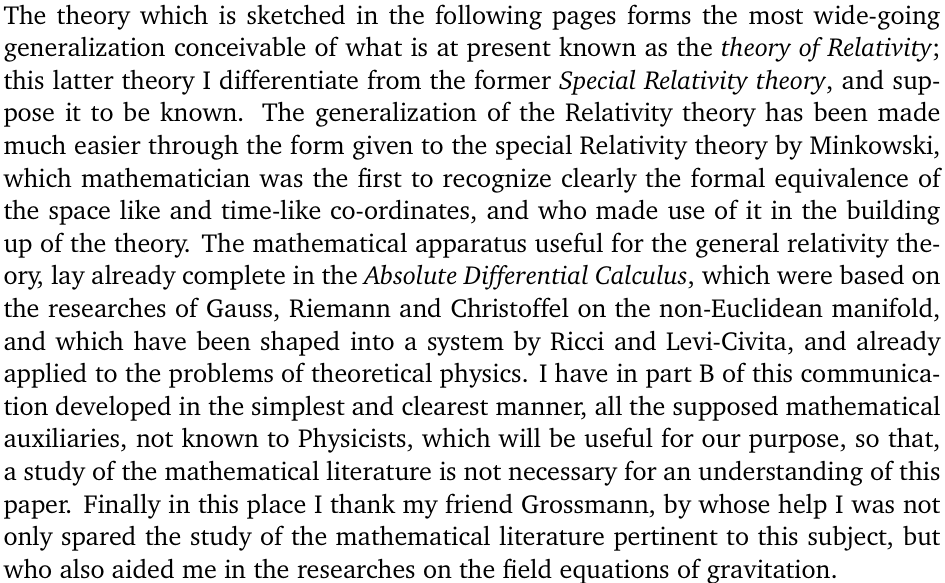
\includegraphics[width=.95\columnwidth]{microtype_off.png}}
  \vspace{0pt}
  \subcaption{Text typeset without using \pkg{microtype}.}
  \par\bigskip
  \fbox{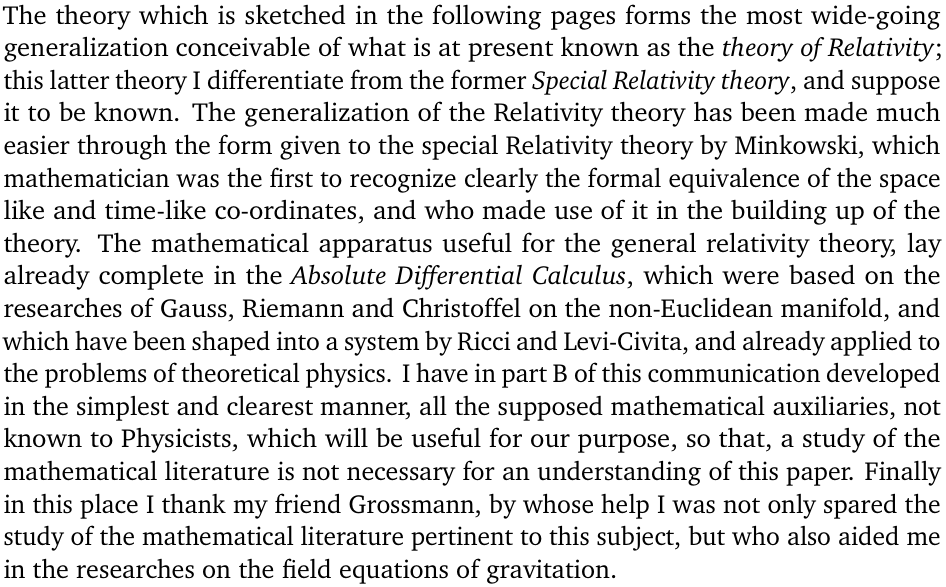
\includegraphics[width=.95\columnwidth]{microtype_on.png}}
  \vspace{0pt}
  \subcaption{The same text typeset using \pkg{microtype} (character
    protrusion \& font expansion).}
  \caption[The effect of using the \pkg{microtype} package.]{The effect of
    using the \pkg{microtype} package. These examples are based on
    \url{https://gist.github.com/AndiH/8b65adbeb77b00c4b970}.}
  \label{fig:microtype}
\end{figure}
It works best with \prog{pdflatex} or \prog{lualatex}.

LaTeX is basically a document processing system for text. The easiest way to
include graphics or diagrams, is to generate them with an external processor
and then include them with `\verb"\includegraphics"'\,\footnote{This command is
  defined by the \pkg{graphicx} package, which is already preloaded by the
  \cls{kulemt} class.}. But external processors mostly use different fonts and
scaling, which clashes with the look of the rest of your document. An
alternative is to use the \pkg{tikz} package\,\cite{pkg:tikz} where drawing is
done using TeX commands, such as in \fref{fig:compile}. Its manual of more than
1300~pages shows how to generate graphics for different domains. Furthermore,
\acro{CTAN} holds more than 150~packages enhancing \pkg{tikz} or making use of
it \cite{CTAN-tikz}.

\section{Selecting fonts}\label{sec:fonts}
The thesis guidelines only give some general hints about fonts, but they don't
enforce specific fonts, except for the title page and the cover page. Not only
a text font must be selected but also a matching math font. Even if you don't
use formulas or equations, a math font is often needed for subscripts or
superscripts.

Two types of font formats can be used: the older Type1 format and the modern
OpenType format (\acro{OTF} or \acro{TTF}). Modern operating system fonts, such
as \texttt{Cambria} on Windows (or the free compatible \texttt{Caladea}) or
\texttt{Geneva} on MacOS, are usually only available in the OpenType format.
Both font formats can be used by \prog{lualatex} and \prog{xelatex} while
\prog{pdflatex} can only use Type1 fonts. A list of available fonts in a
standard LaTeX system can be found in \citewithtitle{fontcatalogue}.

You can select your own combination of fonts using standard LaTeX packages. If
no fonts are defined, the default LaTeX fonts (Latin Modern) are used. Recent
packages are aware of the LaTeX engine you use and automatically switch between
the font formats. Often they also provide suitable math fonts. Some examples
are: \pkg{erewhon} (Utopia based), \pkg{libertinus} (used in this manual),
\pkg{newpx} (Palatino based), \pkg{newtx} (Times based), and \pkg{XCharter}
(Charter based). The wrapper-type package \pkg{fontsetup} may simplify choosing
between OpenType fonts with math counterparts. For more information, have a
look at the documentation of these packages on \acro{CTAN}~\cite{CTAN} or via
\prog{texdoc}~\cite{texdoc}. An almost complete overview of all possibilities
is described in a recent \citewithtitle{companion3}.

\section{Adding a bibliography}\label{sec:bib}
The bibliography can be input as a list in the text, using the
\env{thebibliography} environment. A better way to generate a bibliography is
with the help of the BibTeX programme~\cite{tamethebeast} or the Biber
programme~\cite{pkg:biber}. The latter requires the use of the \pkg{biblatex}
package\,\cite{pkg:biblatex}. The bibliographic data is stored in one or more
bibliographic files (files with extension `\file{.bib}'). Apart from a personal
data file, existing data files can be used for some disciplines.
For more information, please consult the website \citewithtitle[lesson~12
(Citations and references)]{learnlatex}. It will also help you choose between
the BibTeX workflow and \pkg{biblatex}. 

The master's programme guidelines or the thesis supervisor determine which
bibliography style to use. If none is specified, you can choose whichever you
find most suited for your text.

\section{Using \prog{latex}, \prog{pdflatex}, \prog{lualatex} or
  \prog{xelatex}?}\label{sec:engine}
The traditional way to compile a LaTeX file uses the \prog{latex} programme. It
outputs the typeset document to a \file{.dvi} file, which is rather TeX
specific. So usually this is converted to a PostScript file using \prog{dvips}
or a \PDF\ file using \prog{dvips}~+~\prog{dvipdfmx}. However, since every
master's thesis must also be submitted electronically in \PDF~format, there is
no reason to take the PostScript route unless your text depends on packages
which work only with PostScript output, such as \pkg{psfrag} or all kind of
PSTricks packages. But often valid or even better replacements exist, such as
the \pkg{tikz} package\,\cite{pkg:tikz}. Conversion tools may also be available
(e.g., the \pkg{pst-pdf} package).

\begin{figure}
  \newcommand*\pnode[2][]{\path (#2) node[rectangle, draw, thick,
    minimum width=20\unitlength, minimum height=10\unitlength,#1]}
  \newcommand*\fnode[2][]{%
    \draw[thick,#1] (#2) +(-5,5) -- +(5,5) --
      +(5,-5) .. controls +(-2,2)  and +(2,1)  ..
      +(0,-5) .. controls +(-2,-1) and +(2,-2) ..
      +(-5,-5) -- cycle;
    \path (#2) node[rectangle, minimum width=10\unitlength,
                    minimum height=10\unitlength, align=center]}
  \setlength\unitlength{1mm}
  \centering
  \begin{tikzpicture}[x=\unitlength, y=\unitlength, semithick, >=stealth']
    \ttfamily\small
    %% program nodes
    \pnode[align=center]{30,17}(pltx){pdflatex\\lualatex\\xelatex};
    \pnode[dashed,align=center]{80,10}(pbtx){bibtex\\biber};
    %% file nodes
    \fnode{ 5,25}(ftex){.tex};
    \fnode{55,25}(fpdf){.pdf};
    \fnode{55,10}(faux){.aux\\[-1ex]\textrm{\ldots}};
    \fnode[dashed]{102,10}(fbbl){.bbl};
    %% arrows
    \draw[->] (ftex.east) -- ++(5,0) |- ($(pltx.west)+(0,2.5)$);
    \draw[->] ($(pltx.east)+(0,2)$)  -- ++(5,0) |- (fpdf.west);
    \draw[->] ($(pltx.east)+(0,-2)$) -- ++(5,0) |- (faux.west);
    \draw[->] (faux.east) -- ++(4,0) |- (15,2)
              |- ($(pltx.west)+(0,-2.5)$);
    \draw[dashed,->] ($(faux.east)+(4,0)$)  -- (pbtx);
    \draw[dashed,->] (pbtx) -- (fbbl);
    \draw[dashed,->] (fbbl.east) -- ++(5,0) |- (12,0) |- (pltx.west);
  \end{tikzpicture}\medskip
  \caption[Steps to compile a LaTeX file]{Steps to compile a LaTeX file. The
    dashed part is needed only if a bibliography is used. As long as the
    \file{.bbl} file or internal files (\file{.aux}, \file{.toc}, \file{.lof},
    \file{.lot}, \ldots) change, (\file{pdf}/\file{lua}/\file{xe})\file{latex}
    must be invoked again. If you use an intelligent editor, it will tell you
    when an extra iteration is needed.}%
  \label{fig:compile}
\end{figure}
If you want a \PDF~file as a result, it's easier to use \prog{pdflatex}, as
illustrated in \fref{fig:compile}. But \prog{pdflatex} has other advantages
too. It uses the pdfTeX engine, which is an enhanced implementation of the TeX
engine used by \prog{latex}. Therefore more advanced features, such as breaking
hyperlinks (\pkg{hyperref} package) or font expansion (\pkg{microtype}
package), are only possible with the pdfTeX engine. Additionally, the pdfTeX
engine can directly include images in the \acro{JPEG} or \acro{PNG} file format
as well as other \PDF\ files. Simple PostScript (e.g., as generated by
MetaPost) can also be included but general \acro{EPS} (Encapsulated Postscript)
not. You'll have to convert the latter to \PDF\ with the \prog{epstopdf}
programme.

A modern installation also provides the \prog{xelatex} and \prog{lualatex}
programmes, based respectively on the XeTeX and the LuaTeX engine. The XeTeX
engine is derived from the TeX engine and supports almost any system font (cf.\
\Sref{sec:fonts}). The LuaTeX engine is a greatly extended version of pdfTeX
using Lua as an embedded scripting language. Some packages use the Lua
interpreter to perform more complex computations than any other TeX based
engine can do. It also enables \prog{lualatex} to use modern fonts (cf.\
\Sref{sec:fonts}).

When you use a LaTeX-oriented editor or online software, such as Overleaf,
selecting the engines or the programmes to run, can be changed in the settings.

A final word of advice: to avoid errors and text drifting to other places,
don't switch between engines gratuitously.


%%% Local Variables: 
%%% mode: latex
%%% TeX-master: "kulemt"
%%% ispell-local-dictionary: "british"
%%% End: 

\ExplSyntaxOn
\NewDocumentCommand\optionlabel{m}{
  \hspace\labelsep
  \let\oldmeta\meta
  \renewcommand*\meta[1]{{\rmfamily \oldmeta{##1}}}
  \normalfont
  \textsc{Option \exp_args:Nx \int_compare:nNnT {\clist_count:n{#1}} > {1} {s} }
  \c_space_tl
  % Assuming \opt corresponds to \textsf
  `` \group_begin: \sffamily \clist_use:nnnn {#1}
    { \group_end: ''~or~`` \group_begin: \sffamily }
    { \group_end: ''  ,~`` \group_begin: \sffamily }
    { \group_end: ''~or~`` \group_begin: \sffamily }
  \group_end: ''}
\ExplSyntaxOff
\newcommand*\optionlabelnote[1]{\hfill \textit{(#1)}}

\chapter{The LaTeX document class \cls{kulemt}}
\label{cha:kulemt}
The document class \cls{kulemt} can be used to generate a master's thesis text
that conforms to the guidelines of the KU~Leuven Faculty of Engineering
Science.

The document class \cls{kulemt} is actually an extension of the \cls{memoir}
document class\,\cite{pkg:memoir}, which already includes the functionality of
the most useful LaTeX packages. So, before adding or changing some
functionality, you should check the \cls{memoir} manual\,\cite{memman} first.

The default styling of the chapter and section headings is pretty plain. Of
course you can tweak all parameters yourself, but the \cls{memoir} class
provides consistent alternatives using the \cs{headstyles}
command\,\cite[section 6.9]{memman}. For changing only the chapter heading
style, the \cs{chapterstyle} command\,\cite[section 6.5]{memman} is available.
The chapter and headings style used by this document are available in the
\pkg{kulemtx} package, which is part of the \verb"kulemt" bundle. More examples
of chapter styles are available from \cite{memchap}.

\section{Requirements}\label{sec:requirements}
\NewInVersion{2.0}
A LaTeX dated 2018-04-06 with a L3 programming layer dated 2019-04-06 is a
minimal requirement. This L3 programming layer contains important improvements,
such as \acro{UTF-8} as the default input encoding (needed for LuaLaTeX and
XeLaTeX) and the introduction of a rollback concept. Version~2 of the
\cls{kulemt} class has been reimplemented completely using the new programming
layer. In case you still need version~1, you can roll back to the version of
2024-12-16 by starting the preamble with the following line.
\begin{quote}
  \verb"\documentclass["\meta{version 1 class options}\verb"]{kulemt}[=v1]"
\end{quote}

The document class \cls{kulemt} is based on the \cls{memoir} document class.
The minimal version of \cls{memoir} is probably 3.7h (dated 2018-12-12), since
it has been tested with this version (and some newer ones).

The default LaTeX input text encoding is \acro{UTF-8}, which supports all
characters. Furthermore Unicode engines (LuaTeX and XeTeX) only support
\acro{UTF-8}. In case you use another encoding with pdfTeX, you have to
include
\begin{quote}
  \verb"\usepackage["\meta{encoding name}\verb"]{inputenc}"
\end{quote}
at the beginning of the preamble.

\section{The configuration file}\label{sec:ini}
The configuration file contains all information about the masters, their
options and layout features. By keeping this information separated from the
document class code, it can easily be updated yearly by somebody without LaTeX
coding experience.

The syntax of the configuration file is described in \cite[Format of the
configuration file]{pkg:kulemt-code}. As a student, you cannot change this file
unless told so by the master's thesis coordinator of your programme or of the
Faculty.

\NewInVersion{2.0}
The default configuration file is \file{kulemt.ini}. It is not compatible with
the version~1 file \file{kulemt.cfg}. A master specific configuration file can
also no longer be used.

\section{Options}\label{sec:options}
The document class can be customised by the user through options. The
options come in two flavours. A first set of options, called
\emph{document class options}, can only be used as options of the
\cs{documentclass} command.
The reason for having document class options is that an option is needed as a
global option, which can also be used by other packages, or that an option is
used during the initialisation of the class itself. The other options, called
\emph{unrestricted options}, can be used everywhere in the document preamble,
either as option of \cs{documentclass} or as an argument of a \cs{setup}
command.

Many options are specified as ``\meta{key}\texttt{=}\meta{value}''. If the
value contains a comma or a space, it must be enclosed in braces:
``\meta{key}\texttt{=}\marg{value}''. Due to the implementation of LaTeX,
options of the \cs{documentclass} cannot contain commands or spaces, contrary
to the argument of \cs{setup}\label{com:setup}. Therefore it's better to put
all options, except the document class options, in the argument of one or more
\cs{setup} commands. The document preamble can contain multiple
\cs{setup}\marg{optionlist} commands. The \meta{optionlist} is a comma
separated list of options.

Options are processed in the order of appearance. This implies that if options
are given multiple times, the last value survives. However \emph{list options}
do not overwrite a previous value but they accumulate values of that option.

Most of the options are optional, except for the \emph{required} options.
However, when the option \opt{article} is used, all of these options are
optional too.

\subsection{Choosing the basic layout}
The thesis layout is the standard layout and is adopted by default.
\NewInVersion{2.0}
The article layout is the second layout and is selected with the \opt{article}
option. The article layout can be used to typeset additional articles which may
be required by your master's programme.

\begin{labelled}{optionlabel}
\item[article]\optionlabelnote{document class option}\\
  This option switches from the thesis layout to the article layout, as
  provided by the \cls{memoir} class.

  In the article layout, no cover page or front pages are generated, all other
  options are optional and
  \NewInVersion{2.0}
  an additional option \opt{twocolumn} is available.
  That additional option can only be used after the \opt{article} option.
\end{labelled}

\subsection{Selecting the master's programme}
\begin{labelled}{optionlabel}
\item[master=\meta{id\,}]\optionlabelnote{required document class option}\\
  The supported master's programme \meta{id\,}s are defined in the
  configuration file. The currently supported \meta{id\,}s for the Faculty of
  Engineering Science are enumerated in \Sref{sec:mastercfg}.

  The \opt{master} option is used to indicate the master's degree this thesis
  is written for. Only one \opt{master} option can be given in the document,
  which makes it impossible to generate one text for different master's
  degrees, even if it is a common work of two or more students from different
  master's programmes. This scenario was considered too unlikely to support,
  also because each master's programme may have its own additional requirements
  on content and layout.

  Obsolete \meta{id\,} definitions may still be available for printing older
  material. See \Sref{sec:obsoletemasters} for available obsolete \meta{id\,}s.
  Note that an \meta{id\,} may change when it becomes obsolete to avoid
  conflicts with valid \meta{id\,}s.

\item[masteroption=\meta{mo}]\optionlabelnote{unrestricted list option}\\
  This option specifies the option (\Dutch{optie}) or the major topic
  (\Dutch{afstudeerrichting}) of the master's degree. The value \meta{mo} is
  either an abbreviation or a text describing the master's programme option.
  The known master's programme option abbreviations are defined in the
  configuration file. The currently supported option abbreviations for the
  Faculty of Engineering Science are enumerated in \Sref{sec:mastercfg}. If a
  text is used for \meta{mo}, it must start with the appropriate word in lower
  case: ``\texttt{option }\ldots'' (``\texttt{\foreignlanguage{dutch}{optie}
  }\ldots'' or ``\texttt{\foreignlanguage{dutch}{afstudeerrichting} }\ldots''
  in Dutch). Examples of full text can be found in \Sref{sec:mastercfg}. As
  mentioned above, if \meta{mo} contains spaces, you cannot use this as a
  document class option.

  Whether or not a master's programme option must be specified depends on your
  master's programme guidelines. Some master's programmes even do not allow you
  to print an option on the title page. You can find all this information in
  \Sref{sec:mastercfg}.

  An error is raised if the master's programme requires you to specify an
  option and \opt{masteroption} is not used. An error is also raised
  if you use \opt{masteroption} and your master's programme disallows options.

  If students from different master's programme options together produce a
  single text, \opt{masteroption} can be used multiple times and the different
  \meta{mo}s are accumulated.

  Obsolete master's programme options may still be available for printing older
  material. Available obsolete options are listed in \Sref{sec:mastercfg}. Note
  that abbreviations may change when they become obsolete to avoid conflicts
  with valid options.
\end{labelled}

\subsection{Declaring the language(s)}
The commands of the \pkg{babel} package can be used to select a language.
Currently only Dutch and English are supported as text language, but other
languages can be used for short fragments of text.
\NewInVersion{2.0}
Additionally British is available, since this is the English variant
recommended by the KU~Leuven. The master's programme language is defined by the
master's degree itself, so it cannot be chosen.

Some engines, such as pdfTeX and XeTeX, use preloaded hyphenation patterns. For
these engines TeX will raise an error if the Dutch hyphenation patterns are not
preloaded in your TeX installation and you use the option \opt{dutch} or the
master's programme language is Dutch. In that case you have to update your
installation.

\begin{labelled}{optionlabel}
\item[dutch, english, british]\optionlabelnote{document class option}\\
  These options select the text language, either English (or its variant
  British) or Dutch. The options are mutually exclusive: at most one of the
  options can be used. If none of the options is used, the text language is set
  to the master's programme language, defaulting to English if no \opt{master}
  option is given.

  Since these options are document class options, they are global LaTeX
  options. This means that other packages which are language sensitive will
  also use these options.

\item[extralanguage=\meta{lang}]\optionlabelnote{document class list option}\\
  To switch the language of text fragments, commands such as
  \cs{foreignlanguage} are available from the \pkg{babel} package. In older
  versions of \pkg{babel} (before version 3.39 dated 2020-02-03) these
  languages must have been defined before they can be used. By default only the
  text language and the master's programme language are defined. If other
  languages are needed with the older versions of \pkg{babel}, they must be
  declared with this \opt{extralanguage} option. The \meta{lang} can be any
  language known to \pkg{babel}, but keep in mind that \pkg{babel} cannot
  handle dialects of a previously defined language.

  If multiple languages must be declared, you have to use this option
  several times.

  With recent versions of \pkg{babel} the \opt{extralanguage} option becomes
  obsolete.
\end{labelled}

\subsection{Information for the title page}
These options provide the necessary information for the title page. Since this
page must be present in the thesis, most of the options are required.

Due to implementation restrictions, math is not supported on the front pages
(although it may work for some fonts). Since you cannot use math in the
metadata you have to submit with the \PDF~file, try to avoid math in the
next options anyway.

\begin{labelled}{optionlabel}
\item[title=\meta{title}]\optionlabelnote{required unrestricted option}\\
  This option provides the official title \meta{title} of the thesis. It
  must be written in the text language, which may be different from the
  master's programme language.

\item[subtitle=\meta{stitle}]\optionlabelnote{unrestricted option}\\
  A subtitle \meta{stitle} is optional. It is only used on the cover and
  the title page. It will not be used in any bibliographic reference.

\item[author=\meta{authors}]
  \optionlabelnote{required unrestricted option}\label{opt:author}\\
  This option provides the name \meta{authors} of the author(s) of the
  thesis. The name consists of a non-abbreviated first name followed by the
  last name without a comma in between. If the thesis text has multiple
  authors, they are all listed in \meta{authors}, separated by the command
  \cs{and}.

\item[promoter=\meta{promoters}]
  \optionlabelnote{required unrestricted option}\\
  This option lists the \meta{promoters} (a.k.a.\ thesis supervisors). If
  the thesis has multiple supervisors and/or co-supervisors, they are all
  listed in \meta{promoters}, separated by the command \cs{and}. The names of
  the supervisors are preceded by their title unless stated otherwise in
  the master's programme guidelines.

  The \meta{promoters} value also lists the co-supervisors. Co-supervisors are
  always given after the supervisor(s). Nothing is provided to differentiate
  between supervisors and co-supervisors. However your master's programme may
  have additional guidelines about this.

\item[promotor=\meta{promoters}]\mbox{}\\
  This option is an alias for the option ``\opt{promoter}''.

\item[assessor=\meta{assessors}]
  \optionlabelnote{required unrestricted option}\\
  This option lists the \meta{assessors} of the thesis separated by the command
  \cs{and}. The names of the assessor are preceded by their title unless
  stated otherwise in the master's programme guidelines. For assessors from
  other universities or companies, their affiliation can be mentioned if the
  master's programme guidelines require it.

  If you do not have any assessor, contrary to the faculty rules, you must use
  this required option but with an empty value for \meta{assessors}, e.g., use
  ``\verb"assessor="'' as an option.

\item[assistant=\meta{assistants}]
  \optionlabelnote{required unrestricted option}\\
  This option lists the \meta{assistants} (a.k.a.\ assistant-supervisors) of
  the thesis separated by the command \cs{and}. For assistants from other
  universities or companies, their affiliation can be mentioned if the master's
  programme guidelines require it.

  If you worked without the help of an assistant, you can use this required
  option with an empty value for \meta{assistants}, e.g., use
  ``\verb"assistant="'' as an option.

\item[acyear=\meta{acyear}]\optionlabelnote{unrestricted option}\\
  This option sets the (starting year of the) academic year the master's degree
  is obtained.
  \NewInVersion{2.0}
  Since version~2, the value \meta{acyear} is a 4-digit number.

  The default is the current academic year. If run after 1~October, the current
  year defines the start of the academic year. Otherwise it defines the end of
  the academic year. So this option should probably only be used in case of
  emergency because the default works quite well.
\end{labelled}

\subsection{Conditionally generating pages}
The options in this section determine which pages are available in the
output file.

\begin{labelled}{optionlabel}
\item[coverpageonly]\optionlabelnote{unrestricted option}\\
  If this option is used, only the title page (which can be used as a cover
  page) is printed. This option supersedes any other option from this section.

\item[frontpagesonly]\optionlabelnote{unrestricted option}\\
  If this option is used, only the front pages (the title page and the
  copyright page) are printed instead of the entire document. You can use this
  option to generate these pages when you are using other text processing
  software to write your thesis.
\end{labelled}

\subsection{The layout of the typeblock}
These options customise the layout of the text area on the page. Most of
them are options available to all traditional LaTeX document classes.

\begin{labelled}{optionlabel}
\item[10pt, 11pt]\optionlabelnote{document class option}\\
  The default font size of the main text can be set to 10\,pt or 11\,pt.
  The options are mutually exclusive. The default size is 11\,pt.

  All other fonts used in the text are scaled proportionally. Additionally
  the line width of a 10\,pt text is decreased by 1\,cm because of
  readability reasons.

\item[oneside, twoside, twosidelrequal]%
  \optionlabelnote{document class option}\\
  These mutually exclusive options declare where the typeblock will be located
  and whether the document will be printed on both sides of the paper or only
  on one side. The default value is \opt{twosidelrequal}, so you only need it
  to cancel a previous option \opt{oneside} or \opt{twoside}.

  The \opt{twoside} option indicates that the text will be printed on both
  sides of the paper. By default, each main chapter starts on a recto page (the
  right-hand page of the printed book). To get a more pleasing look, the inner
  margins (right on verso, left on recto) are smaller than the outer margins,
  as shown on \fref{fig:spread}.
  \begin{figure}
    \centering
    \setlength\unitlength{.5pt}
    \newcommand*\typeblock[1]{%
      \draw[thin] (#1) rectangle +(140,215);
      \draw[thin] (#1) -- +(140,215);
      \draw[thin] (#1) +(0,215) -- +(140,0);
    }
    \begin{tikzpicture}[x=\unitlength, y=\unitlength]
      \draw[thick] (0,0) rectangle (410,297); % page spread
      \draw[thick] (210,0) -- +(0,297); % page border
      \typeblock{45,45}   % LH typeblock
      \typeblock{235,45}  % RH typeblock
    \end{tikzpicture}\medskip
    \caption{In a spread, showing a left verso and a right recto page, the
      combination of the two inner margins is perceived as a single margin.
      Therefore the width of an outer margin is comparable to two times the
      width of an inner margin.}
    \label{fig:spread}
  \end{figure}

  The \opt{oneside} option indicates that it either will be printed on one side
  or it will be available for on-screen viewing only. Contrary to printed
  books, electronic versions are usually read from the screen, one page at a
  time. In the latter case it makes more sense to have equal left and right
  margins and to avoid empty pages between chapters. The latter can be obtained
  by allowing chapters to begin on any page, not only on odd numbered pages.

  \NewInVersion{2.0}
  If your thesis will primarily be distributed for on-screen viewing, but it
  should also look nice when printed, you can use the option
  \opt{twosidelrequal}. This is equivalent to the \opt{twoside}
  option, but with equal inner and outer margins. This way the typeblock
  does not jump from left to right when you page on-screen through the thesis.

  The \cls{kulemt} document class has been designed to guarantee that the size
  of the typeblock does not change when you switch between the options, only
  its horizontal position. This means that you can without problems use the
  \opt{twoside} option to generate the high quality printed version and the
  \opt{twosidelrequal} option for the \PDF\ version.

  \NewInVersion{2.0}
  To keep life easy, \opt{twosidelrequal} is the new default since
  version~2. To revert to the default of version~1, you must explicitly use
  the \opt{twoside} option.

\item[openright, openleft, openany]
  \optionlabelnote{document class option}\\
  These options determine the page on which a new chapter in the main
  matter starts.
  \begin{itemize}
  \item \opt{openright}: Each main matter chapter starts on a recto page. This
    is customary in printing.
  \item \opt{openleft}: Each main matter chapter starts on a verso page. Only
    use this if your supervisor demands it.
  \item \opt{openany}: A main matter chapter can start on any page. You can use
    this to remove empty pages between chapters.
  \end{itemize}

  The three options are mutually exclusive. The default value is
  \opt{openright}. For one-side printing only recto pages are used, so
  these options are irrelevant.

  The \cls{memoir} class also provides the \cs{openright}, \cs{openleft},
  and \cs{openany} commands to change this inside the document itself.

\item[bind=\meta{binding length}]\optionlabelnote{document class option}\\
  When you open a two-side printed book, some paper of the inner margins is
  invisible due to the binding of the book. It seems as if the inner
  margins are smaller than specified. This option specifies the amount
  \meta{binding length} of the invisible inner margin of a page. This amount
  is specified as a length (e.g., \opt{3mm}) and it defaults to
  0\,mm.
\end{labelled}

\subsection{Other options}
\begin{labelled}{optionlabel}
\item[cfgfile=\meta{file}]\optionlabelnote{document class option}%
  \NewInVersion{2.0}\\
  This option lets you use another configuration file \meta{file} instead of the
  standard file \file{kulemt.ini}. 

\item[draft]\optionlabelnote{document class option}\\
  The \opt{draft} option is a global option which influences many packages.
  The main effect is to mark overfull lines and to not show graphics content.

\item[fleqn]\optionlabelnote{document class option}\\
  By default displayed math equations are centred. Using this option puts all
  displayed equations at the left margin, indented by an amount of
  \cs{mathindent}.

\item[oldfontcommands]\optionlabelnote{document class option}\\
  The \opt{oldfontcommands} option is passed to \cls{memoir} to make the old,
  deprecated LaTeX version 2.09 font commands available. Please use this only
  to solve problems with old packages you are forced to use.
\end{labelled}

\subsection{Options removed in version 2}
\NewInVersion{2.0}
The following version~1 options are no longer available. Using them results in
errors.

\begin{itemize}
\item The option \opt{font} has been removed. If you prefer other fonts than
  the default ones, you have to load the appropriate packages yourself (cf.\
  \Sref{sec:fonts}).
\item The option \opt{inputenc} has been removed. If you insist on using an
  encoding different from \acro{UTF-8} with pdfTeX, you have to load the
  \pkg{inputenc} package yourself (cf.\ \Sref{sec:requirements}).
\item Since a filing card is no longer provided, the option `\opt{filingcard}'
  is removed as well as all options providing additional information for the
  filing card: \opt{translatedtitle}, \opt{shortabstract}, \opt{udc},
  \opt{keywords}, and \opt{articletitle}.
\item The package \pkg{microtype} is no longer loaded automatically by the
  \cls{kulemt} class, so the option \opt{nomicrotype} becomes irrelevant and is
  removed.
\item The option \opt{bindcover} has already been obsolete since version~1.7,
  so it is removed.
\end{itemize}


\section{Additional commands and environments}
The (extensive) basic functionality of the \cls{memoir} class, complemented
by existing LaTeX packages, provides most of the commands to write a master's
thesis according to the guidelines. This section describes the additional
commands and environments defined by the \cls{kulemt} class to extend the
user capabilities.

One of the new commands is \cs{setup}\marg{optionlist}. It is used to set
options with values which contain other commands. This command is described
on page~\pageref{com:setup}.

\subsection[\env{preface}]{The \env{preface} environment}
The \env{preface} environment contains the preface text to be typeset on
the preface page.

The environment has one optional argument, which holds the preface author. It
defaults to the value of the \opt{author} option (cf.\
page~\pageref{opt:author}). This argument is typeset at the right margin in
italics after the preface text. The argument can be used to remove the preface
author (by providing an empty argument) or to add information such as a date to
it. Just try out the following example right after \verb"\begin{document}":
\begin{verbatim}
  \begin{preface}[The Author\\ \textup{1 January 2010}]
    The text of the preface. A few paragraphs should follow.
  \end{preface}
\end{verbatim}

\subsection[\env{abstract*}]{The \env{abstract*} environment}
The existing \env{abstract} environment typesets an abstract page in the
text language. An additional \env{abstract*} environment is defined to
typeset an additional abstract page in another language.
%\NewInVersion{1.6}
The language of the \env{abstract*} environment is given in the optional
argument. It defaults to the official master's programme language. It is
typically used to add an additional abstract page if the thesis is written in a
language different from the master's programme language.

\subsection[\cs{listoffiguresandtables}]{%
  The \cs{listoffiguresandtables} command}
Normally all ``List of \ldots'' overviews are printed on a separate page.
However, for shorter texts like a master's thesis these lists may be smaller
than half a page. Therefore an additional command
\cs{listoffiguresandtables} is provided, which combines the list of
figures and tables without a page break.

The list of figures and tables are put in separate sections of one chapter,
first the figures then the tables. The command
\cs{listfiguresandtablesname} holds the title of the chapter.


%%% Local Variables: 
%%% mode: latex
%%% TeX-master: "kulemt"
%%% ispell-local-dictionary: "british"
%%% End: 


\appendix
\appendixpage*

\chapter{Information about the master's programmes}

\ReadConfigFile

This \ifanappendix appendix \else chapter \fi gives an overview of the master's
programmes of the Faculty of Engineering Science. These master's programmes are
supported by default by the LaTeX document class \cls{kulemt}. But all of this
information is also valid for non-LaTeX documents.

\section{Information from \file{\ConfigFileName}}
\label{sec:mastercfg}
The master's programme specific information is stored in the
\file{\ConfigFileName} file. It contains information about the master's
programme language, the programme's faculty, known master's programme options,
and copyright contact information.

\ifdefined\microtypesetup \microtypesetup{protrusion=false}\fi

This section describes the \file{\ConfigFileName} file dated
\PrintConfigFileDate. For the latest information, consult
\file{\ConfigFileName} directly.
If no faculty name is shown, it is an inter-faculty programme.

\subsection{Dutch initial master’s programmes}
\PrintMastersInfo{initial}{dutch}

\subsection{English initial master’s programmes}
\PrintMastersInfo{initial}{english}

\subsection{Advanced master’s programmes}
\PrintMastersInfo{advanced}{}

\subsection{Obsolete master’s programmes}
\label{sec:obsoletemasters}
\PrintMastersInfo*{}{}

%%% Local Variables: 
%%% mode: latex
%%% TeX-master: "kulemt"
%%% ispell-local-dictionary: "british"
%%% End: 

\newcommand*\showtemplatefile[1]{%
  \begingroup
    \setverbatimfont{\normalfont\ttfamily\footnotesize}%
    \bvperpagefalse
    \linenumberfrequency{1}\resetbvlinenumber
    \linenumberfont{\rmfamily\tiny}%
    \bvnumbersoutside
    \renewcommand*\bvtoprulehook{%
      \hrule width\linewidth \nobreak
      \hbox to\linewidth{%
        \hss \smash{\colorbox[gray]{.9}{%
            \ttfamily \enspace template/#1\enspace}}\qquad}%
      \nobreak\vskip-.1pt\nobreak\vskip-\lineskip\relax}%
    \boxedverbatiminput{#1}%
    \tracingnone
  \endgroup}

\chapter{LaTeX Template}
\label{app:template}
LaTeX templates are provided for a Dutch master's programme as well as for an
English one. The Dutch and English examples can be found respectively in the
directories `\file{sjabloon}' and `\file{template}' of the documentation
directory (the directory where the file you're reading is installed). For each
main file (either \file{masterproef.tex} or \file{thesis.tex}) the resulting
typeset \PDF\ file is available as a reference.

The following sections give examples of the most important files of the
template: the main file (\Sref{sec:file:main}), a sample chapter
(\Sref{sec:file:chap}), and the bibliography database (\Sref{sec:file:bib}).
Translated versions for a Dutch master's programme can be found in the directory
`\file{sjabloon}'. Finally \Sref{sec:file:hoofd} gives an example of a main
file for a Dutch master's programme but written in English.

All the examples below use the \pkg{lipsum} package to generate dummy text.
Of course this is only needed as an example to quickly generate a lot of
text. Because you will never need it in your real text, you can start by
removing all invocations of \cs{lipsum} in all files as well as the lines
20--27 of the main files (\Sref{sec:file:main} and \Sref{sec:file:hoofd}).

\section{The main file}
\label{sec:file:main}
\showtemplatefile{thesis.tex}

\section{A sample chapter}
\label{sec:file:chap}
\showtemplatefile{chapter-1.tex}

\section{The bibliography database}
\label{sec:file:bib}
\showtemplatefile{references.bib}

\section{The main file of an English text for a Dutch master's programme}
\label{sec:file:hoofd}

The main differences between an English text for an English master's programme
(\Sref{sec:file:main}) and an English text for an Dutch master's programme are:
\begin{itemize}
\item the use of the \opt{english} option (line~1);
\item an additional \env{abstract*} environment is needed (lines 51--59).
\end{itemize}
\medskip

\showtemplatefile{thesis-dutch.tex}

%%% Local Variables: 
%%% mode: latex
%%% TeX-master: "kulemt"
%%% ispell-local-dictionary: "british"
%%% End: 


\backmatter
\newenvironment{termlist}%
 {\renewcommand*\descriptionlabel[1]{\hspace\labelsep
    \normalfont\scshape ##1}%
  \let\olditem\item
  \renewcommand*\item[1][??]{\olditem[##1]\leavevmode\newline\ignorespaces}%
  \newcommand*\latex{\unskip\quad\upshape (LaTeX)}%
  \description}%
 {\enddescription}

\chapter{Terminology}
\label{cha:terminology}
\begin{termlist}
\item[Back matter]
  The back matter conveys information ancillary to that in the main matter,
  such as a bibliography, an index, or a glossary.
\item[Copyright page]
  Second (unnumbered) page of the thesis, containing the copyright
  statements. It is part of the front pages.
\item[Cover page]
  The cover page (\Dutch{kaft} in Dutch) will be printed on the front of the
  hard cover of your booklet. Although it is part of the front pages, it is not
  part of the printed or electronic thesis. It is generated separately.
\item[Document class option \latex]
  A document class option can only be used as an option of the
  \cs{documentclass} command.
\item[Engine \latex]
  In TeX parlance, the engine is the programme which compiles the TeX document
  using a macro package. Several engines currently exist: TeX (the original by
  D.\ Knuth, outputting \file{.dvi}), eTeX (TeX with some extended
  capabilities), pdfTeX (extended eTeX and additional \PDF\ output), XeTeX
  (eTeX which can use system fonts), and \mbox{LuaTeX} (scriptable pdfTeX). All
  these engines can preload the LaTeX macro package. On modern systems,
  \file{latex} means pdfTeX in compatibility mode (equivalent to the TeX
  engine) with LaTeX preloaded and \file{pdflatex} means pdfTeX with LaTeX
  preloaded (generating \file{.pdf} output). The commands \file{xelatex} and
  \file{lualatex} run respectively the engine XeTeX or LuaTeX with LaTeX
  preloaded.
\item[Font]
  A font is a set of visual representations of characters in a specific
  typeface.
\item[Font family]
  A font family is a set of fonts designed to work harmoniously together.
  Typically this means at least a roman font and an italic font. But it can
  be extended to combinations of serif and sans-serif fonts.
\item[Front matter]
  The front matter is the part of the thesis, which contains the
  introductory material such as a preface, an abstract, and content lists
  (table of contents, list of tables, list of figures, list of symbols, etc.).
\item[Front pages]
  In this text the front pages refer to the title page and the copyright page.
\item[Leading]
  Leading is the vertical space between two lines of text. The line spacing
  is the font size plus the leading.
\item[Main matter]
  The main matter is the middle part of the thesis, between the front and
  the back matter. It contains the actual information of the thesis in
  regular chapters and appendices.
\item[Master's programme language]
  The master's programme language refers to the official language of the
  master's programme. Usually it is the same as the text language but not
  necessarily.
\item[Optical alignment of margins]
  Some characters (e.g., punctuation) can make a line appear shorter than
  others to the human eye. Shifting such characters by an appropriate
  amount into the margins (called character protrusion) gives the impression
  that the margins are aligned and not ragged.
\item[Point (pt)]
  A point (pt) is a printer's unit: $72.27\,\mathrm{pt} = 1\,\mathrm{inch} =
  25.4\,\mathrm{mm}$. PostScript and other popular software, such as word
  processors, use a slightly larger point size: $72\,\mathrm{pt} =
  1\,\mathrm{inch}$.
\item[Preamble \latex]
  The document preamble is the part of a LaTeX document, which comes before
  the \verb"\begin{document}" command.
\item[Protrusion]
  See `Optical alignment of margins'.
\item[Recto page]
  The recto page is the right-hand page of a printed book. It normally
  corresponds to odd numbered pages.
\item[Serif]
  A serif is a cross stroke at the bottom of a letter. Compare a serif and
  a sans-serif typeface: ``{\fontfamily{lmr}\selectfont A serif}'' and
  ``{\fontfamily{lmss}\selectfont A sans-serif}''.
\item[Text language]
  The text language refers to the language used to write the text in.
  Usually it is the same as the master's programme language but not necessarily.
\item[Title page]
  The first (unnumbered) page of the thesis. It is part of the front pages.
\item[Typeface]
  A typeface is a visual style to represent characters, regardless of their
  size. This sentence uses the typeface `\rmfontname'. 
\item[Verso page]
  The verso page is the left-hand page of a printed book. It normally
  corresponds to even numbered pages.
\end{termlist}

%%% Local Variables: 
%%% mode: latex
%%% TeX-master: "kulemt"
%%% ispell-local-dictionary: "british"
%%% End: 


\defbibnote{intro}{%
  Local documentation can be accessed from the command line using the
  \prog{texdoc} programme (\prog{mthelp} on a MikTeX installation). That
  local documentation corresponds to the packages installed on your system. The
  most recent documentation can be found online using the \acro{URL}.
  \bigskip
}
\printbibliography[heading=bibnumbered,prenote=intro]

\end{document}

%%% Local Variables: 
%%% mode: latex
%%% TeX-PDF-mode: t
%%% TeX-master: t
%%% ispell-local-dictionary: "british"
%%% End: 
